\subsubsection{Overview}
Data control board (DCB) are intented to be a part of the LHCb upstream tracker
upgrade.
There is one master GBTx ASIC, and 6 data GBTx ASICs per board.
DCB is much less flexible than GBTx DB, because it serves only one purpose:
Receive SALT elink data then transmit that data to the counting room.

So far, we have been able to repeat PRBS test on DCBs:
Programming the master, then programming data GBTxs, then instruct them to
generate PRBS data, and verify generated data by MiniDAQ.

\autoref{fig:dcb_layout} shows the layout of an actual DCB board.
More detailed GBTx ASICs and optical fiber grouping are described in the
caption.

A DCB requires 4 optical mezzanines (not shown here) to function properly.
As said above, DCB is less flexible, and there will be only \emph{one}
configuration for DCBs.
All DCBs shipped with UMD LHCb group will have its hardware jumpers
pre-configured.

\begin{figure}[!ht]
\centering
\begin{tikzpicture}
    \node [anchor=south west] (main) {
            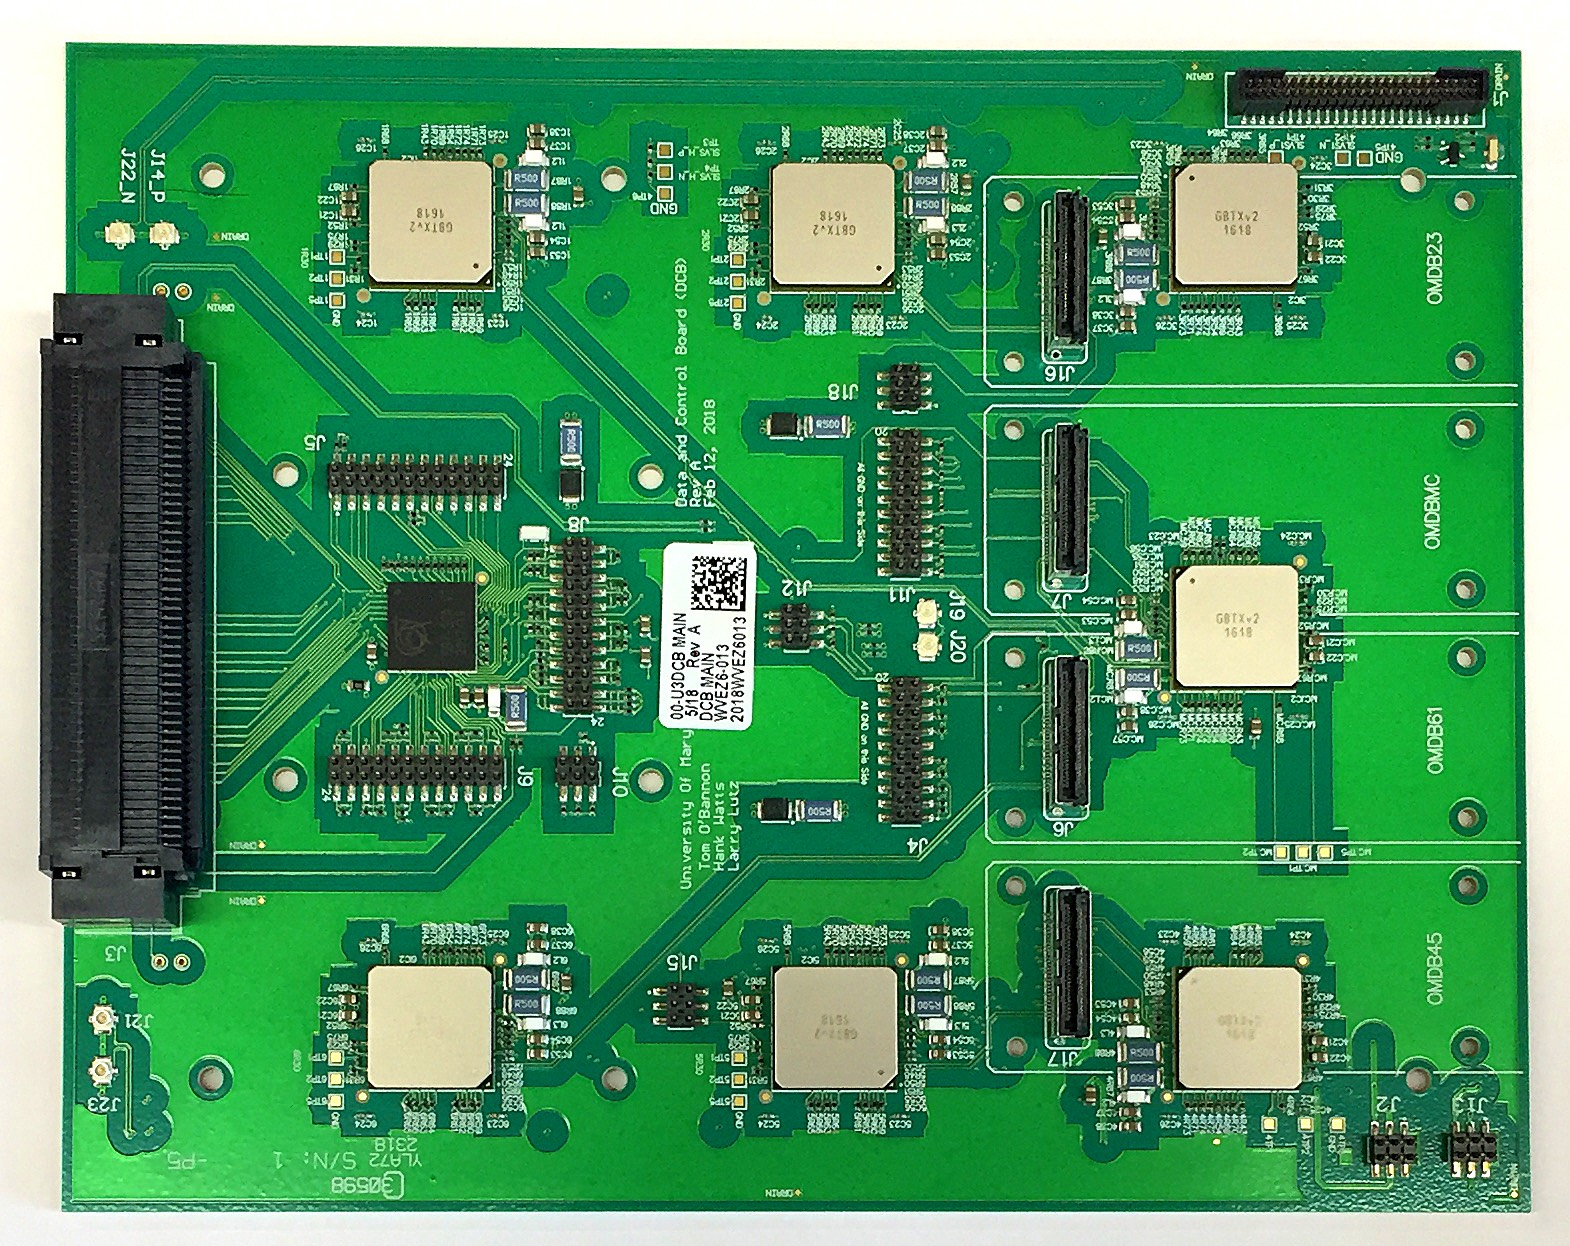
\includegraphics[width=0.9\linewidth]{res/dcb_layout.png}
        };
    \begin{scope}[x=(main.south east),y=(main.north west)]
        \node [draw,red,minimum height=5em,minimum width=2em] (zoombox1)
            at (0.51,0.65) {};
    \end{scope}
\end{tikzpicture}
\caption{
    Currently 007 cannot regain lock, but 008 can.
    Note that during the loss of lock stage, 008 is much more noisy.
    Measured on 008.
}
\label{fig:dcb_layout}
\end{figure}
